\chapter{Лабораторная работа 2}
\section*{Тренировочное задание, вариант 3}

Осуществить планирование проекта со следующими временными характеристиками:

\begin{figure}[h!]
	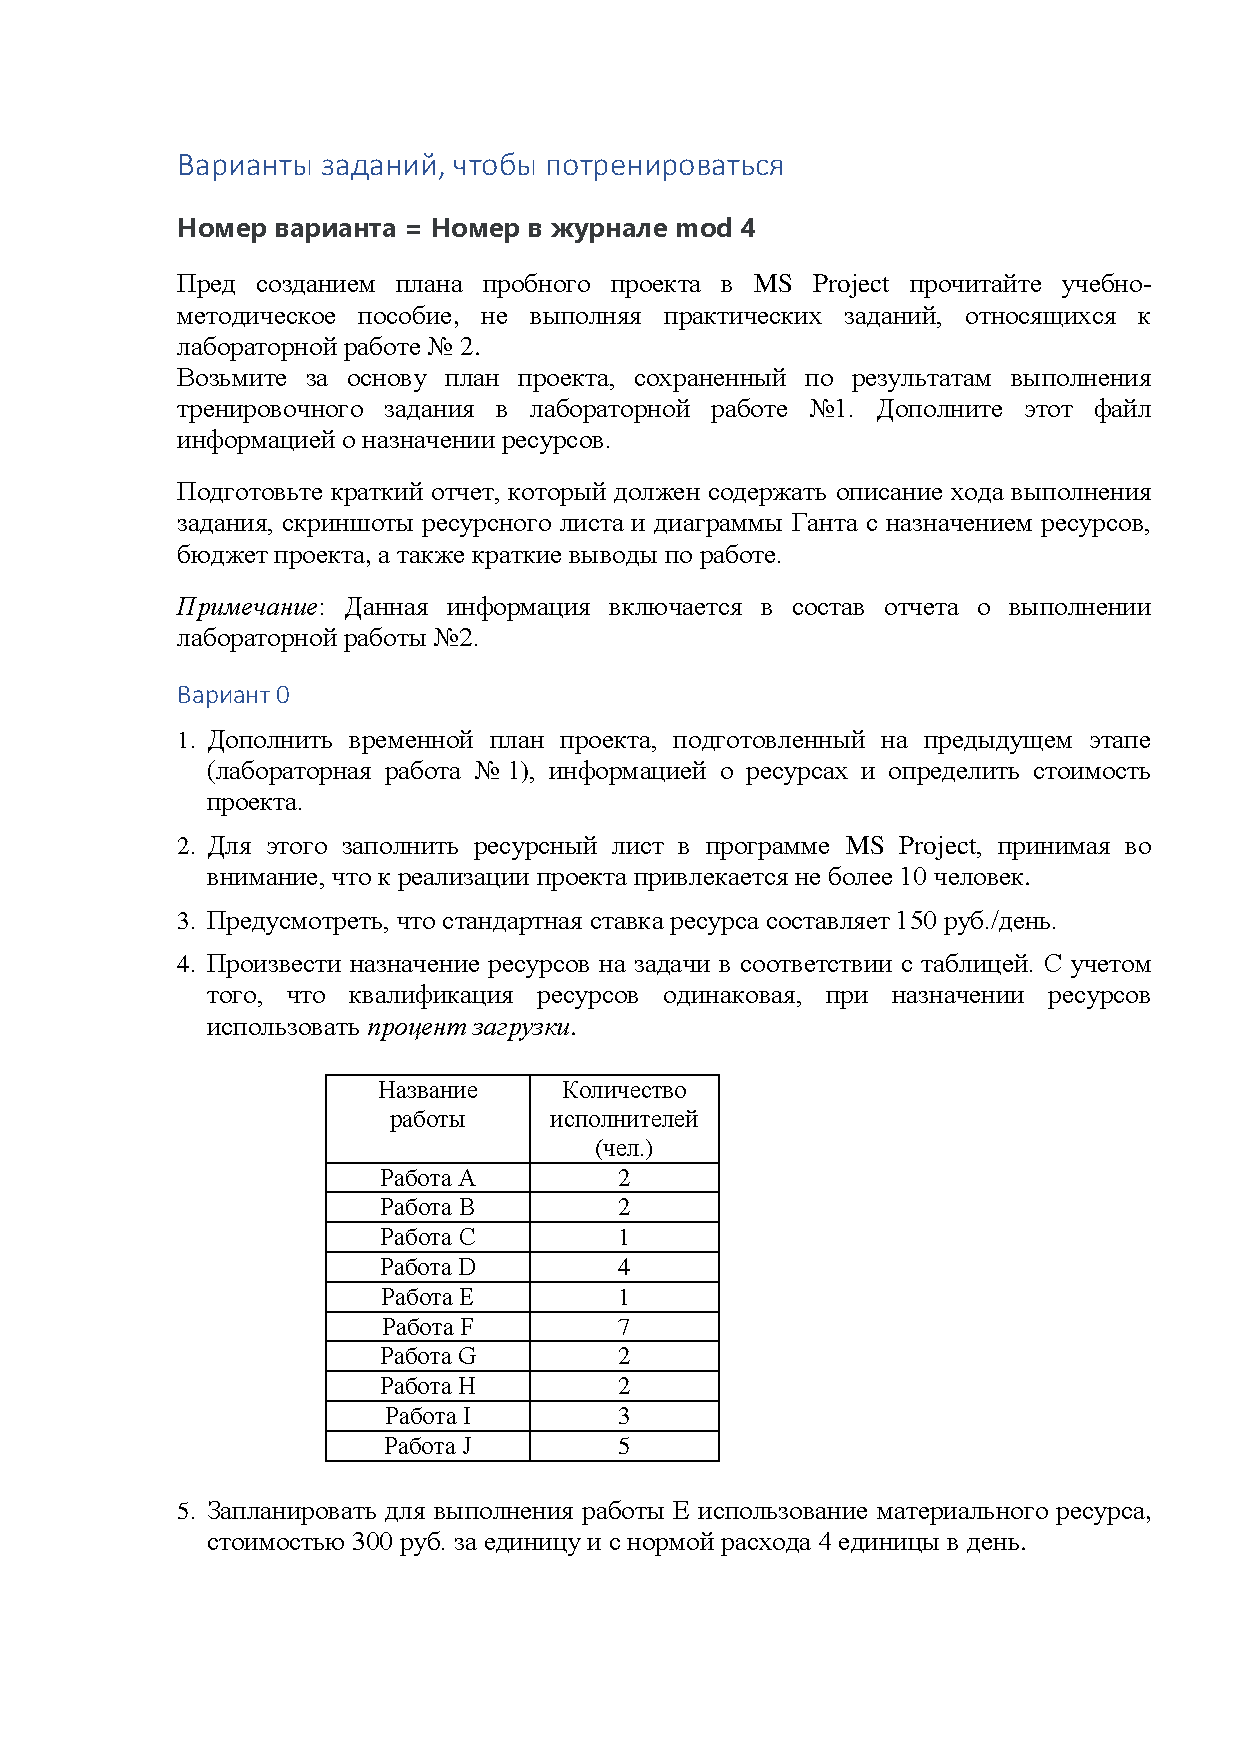
\includegraphics[scale=0.8, center]{lab02_train}
\end{figure}

\begin{enumerate}
	\item Дополнить временной план проекта, подготовленный на предыдущем этапе (лабораторная работа № 1), информацией о ресурсах и определить стоимость проекта.
	\item Для этого заполнить ресурсный лист в программе MS Project, принимая во внимание, что к реализации проекта привлекается не более 10 исполнителей..
	\item Предусмотреть, что стандартная ставка ресурс составляет 200 руб./день.
	\item Произвести назначение ресурсов на задачи в соответствии с таблицей. С учетом того, что квалификация ресурсов одинаковая, при назначении ресурсов использовать процент загрузки.
	\item Для выполнения работ С и Е предусмотреть назначение материального ресурса стоимость 100 рублей за штуку и расходом 2 штуки для работы С и 5 штук для работы Е.
\end{enumerate}

Результат:

\begin{figure}[h!]
	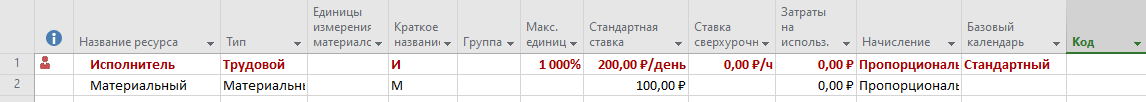
\includegraphics[scale=0.3, center]{lab02_train-result-1}
\end{figure}

\begin{figure}[h!]
	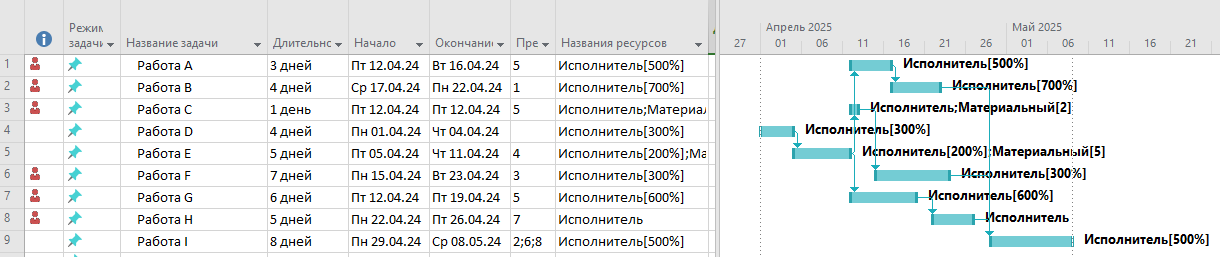
\includegraphics[scale=0.3, center]{lab02_train-result-2}
\end{figure}

Видно, что исполнители перегружены и на некоторые задачи не хватает исполнителей. Общие затраты на проект составляют 34 300 рублей.

\clearpage
\section*{Практическое задание}

Целью лабораторной работы №2 является обучение работе с ресурсами в проекте, созданном в Microsoft Project.

\textbf{Содержание проекта:} команда разработчиков из 16 человек занимается созданием карты города на основе собственного модуля отображения. Проект должен быть завершен в течение 6 месяцев. Бюджет проекта: 50 000 рублей.


\subsection*{Задание 1}

Был заполнен ресурсный лист в соответствии с заданием.

\begin{figure}[h!]
	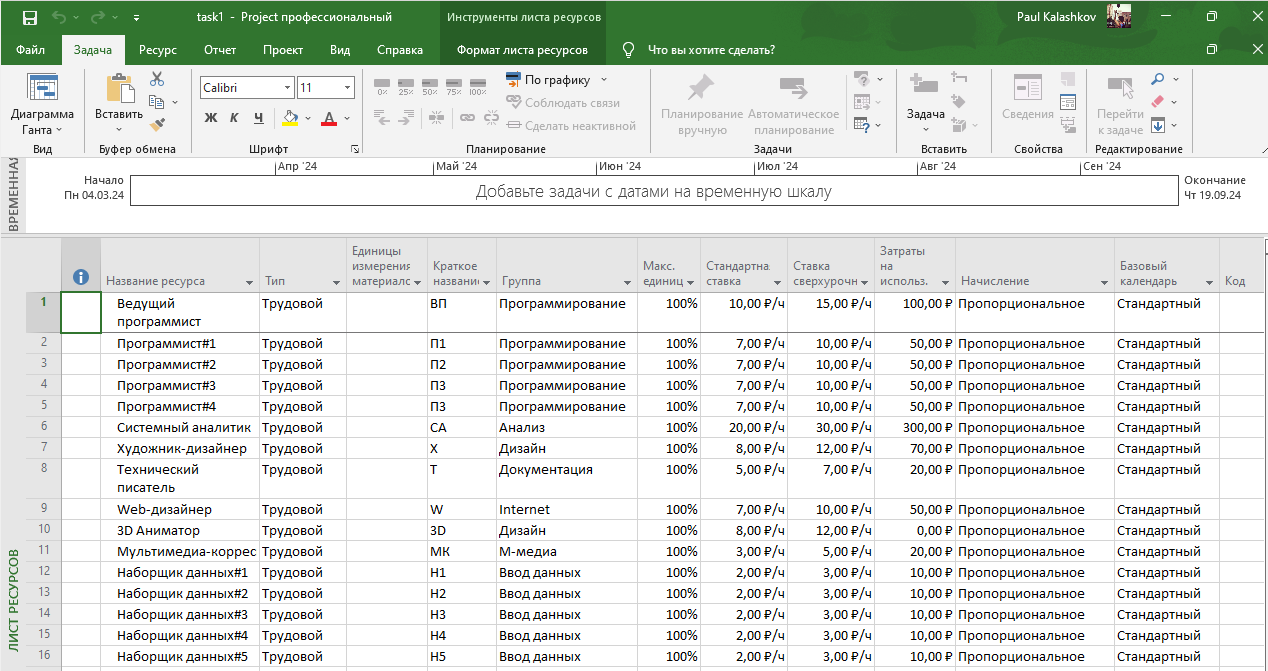
\includegraphics[scale=0.4, center]{lab02_task1}
\end{figure}

\subsection*{Задание 2}

Были назначены ресурсы в соответствии с таблицей.
Исходя из полученных результатов, возникли перегрузки ресурсов, а именно для художника-дизайнера, технического  писателя и системного аналитика. Это происходит из-за того, что системный аналитик параллельно занимается анализом структуры базы данных и анализом ядра, художник-дизайнер одновременно занимается созданием дизайна руководства и разработкой дизайна сайта, а технический писатель --- написанием руководства пользователя и созданием справочной системы (см. ниже).

\begin{figure}[h!]
	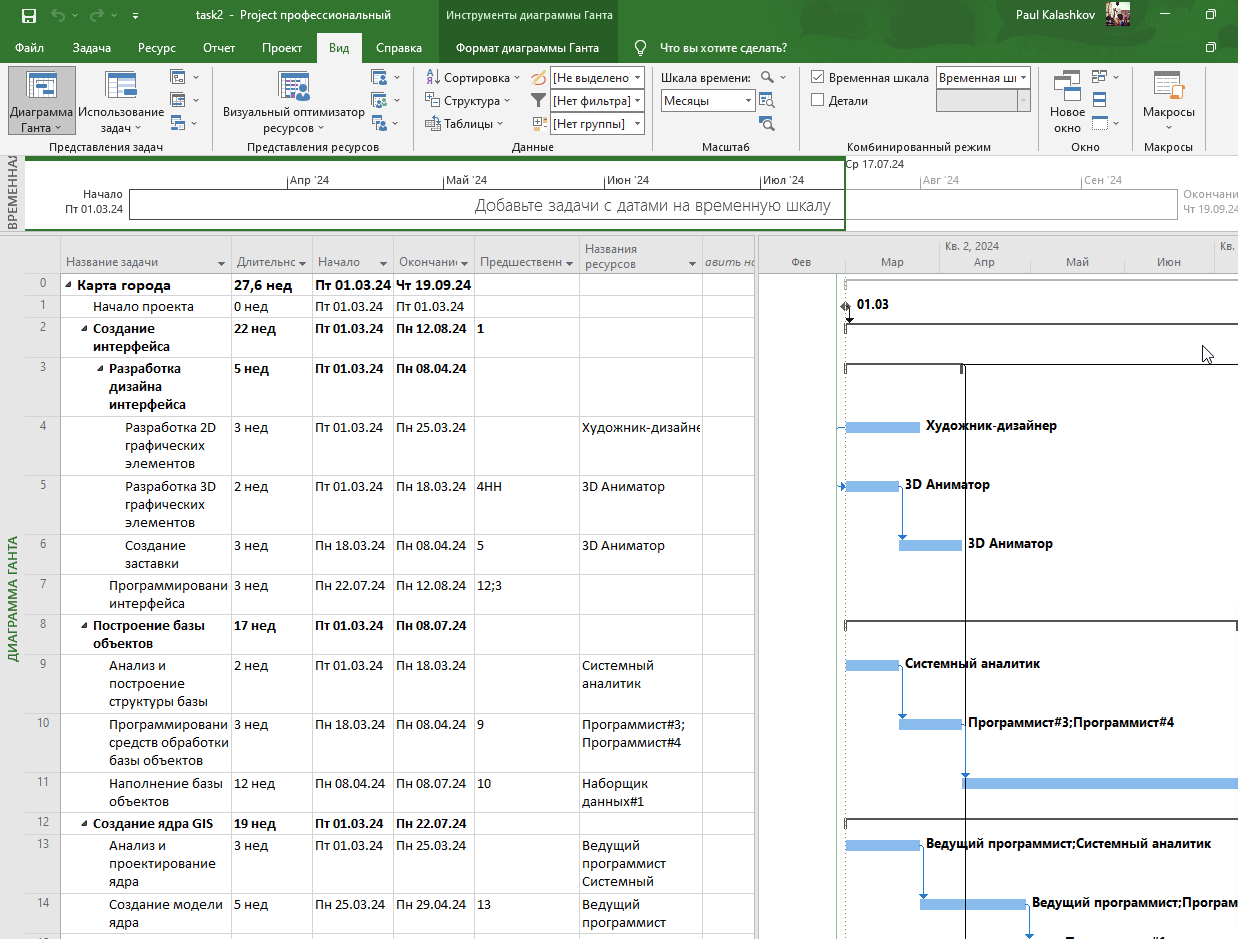
\includegraphics[scale=0.4, center]{lab02_task2_1}
\end{figure}

\begin{figure}[h!]
	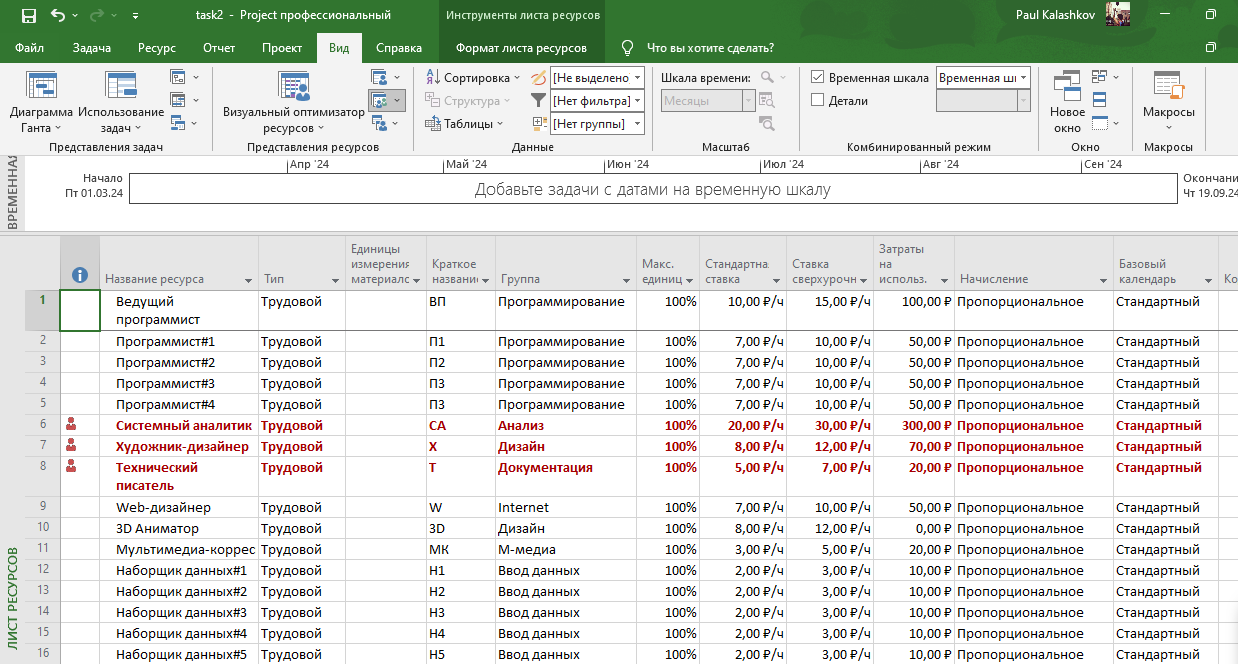
\includegraphics[scale=0.4, center]{lab02_task2_2}
\end{figure}
\clearpage

Продемонстрируем это при помощи оптимизатора ресурсов:

\begin{figure}[h!]
	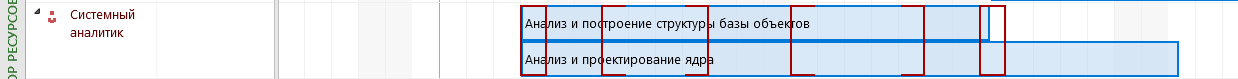
\includegraphics[scale=0.4, center]{lab02_task2_3_1}
\end{figure}

\begin{figure}[h!]
	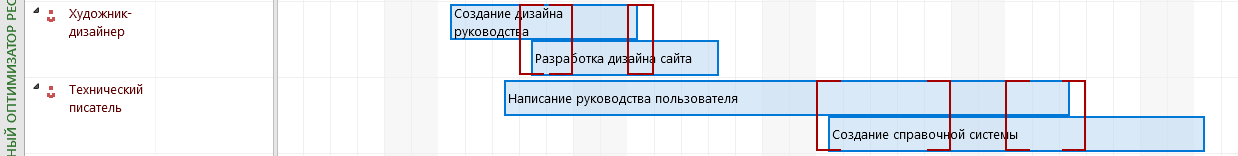
\includegraphics[scale=0.4, center]{lab02_task2_3_2}
\end{figure}

Задачам 2, 8 и 12 были присвоены фиксированные затраты 1000 р.

\begin{figure}[h!]
	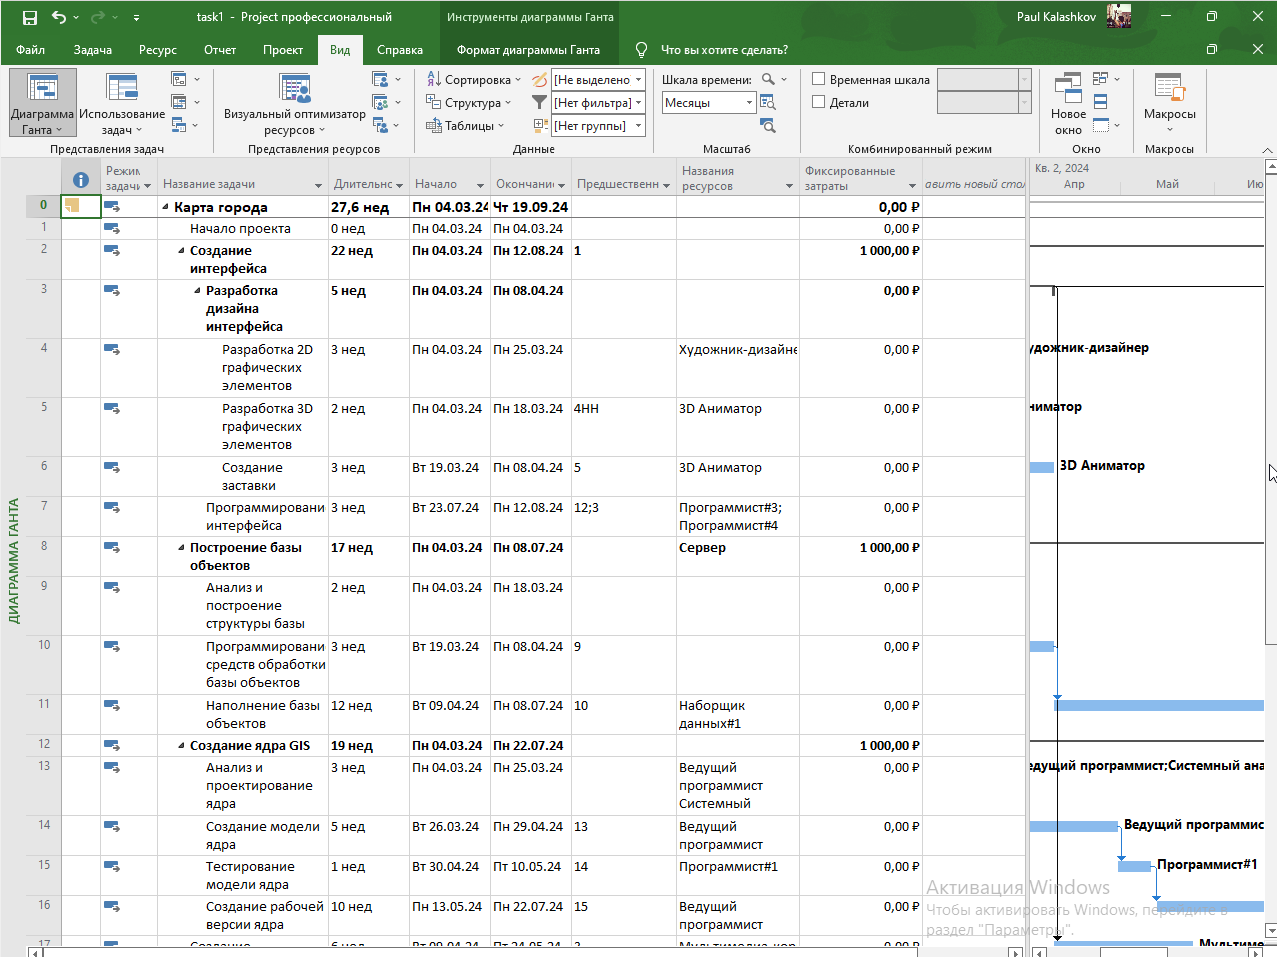
\includegraphics[scale=0.3, center]{lab02_task2_4}
\end{figure}

Для задачи 8 был арендован дополнительный сервер (2 рубля за час). Сервер назначен как трудовой ресурс, потому что стоимость его использования пропорциональна времени. Общая стоимость аренды составила 6 194 рубля.
\clearpage
%\begin{figure}[h!]
%	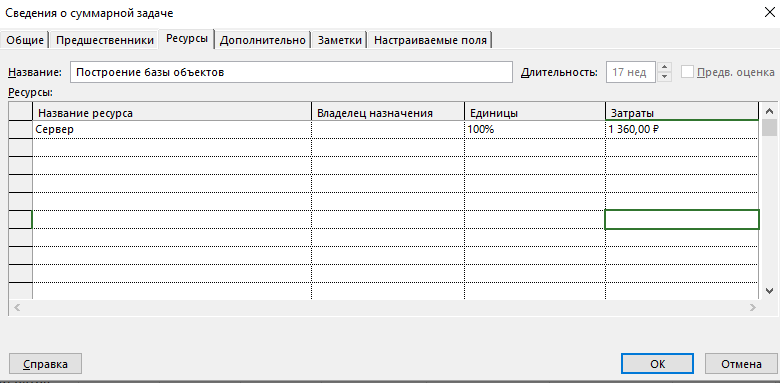
\includegraphics[scale=0.4, center]{lab02_task2_5}
%\end{figure}

\subsection*{Задание 3}

Было получено использование ресурсов с группировкой по группам.
\begin{figure}[h!]
	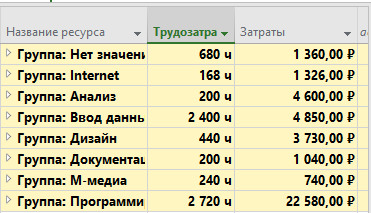
\includegraphics[scale=0.4, center]{lab02_task3_1}
\end{figure}

Были построены диаграммы для расчёта процентного соотношения затрат и трудозатрат.

\begin{figure}[h!]
	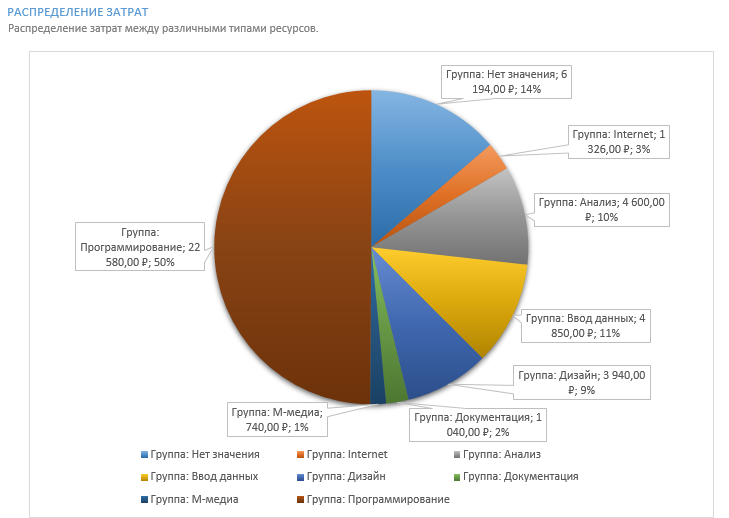
\includegraphics[scale=0.6, center]{lab02_task3_2}
\end{figure}

\begin{figure}[h!]
	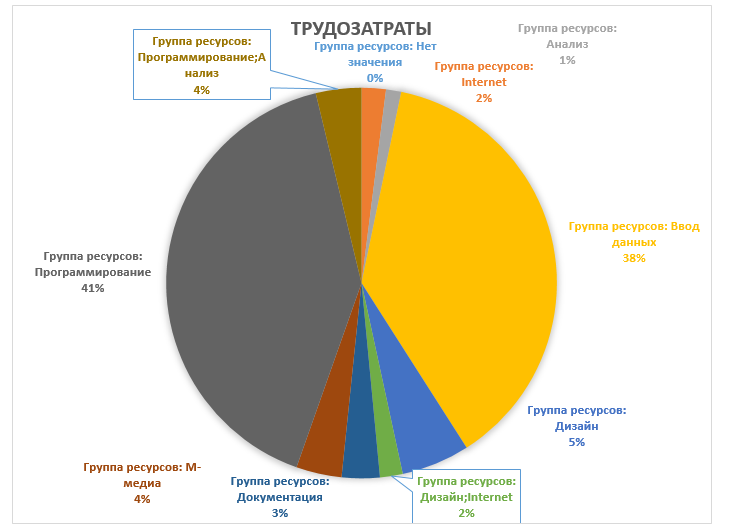
\includegraphics[scale=0.6, center]{lab02_task3_3}
\end{figure}


\clearpage

\section*{Заключение}

В ходе выполнения данной лабораторной работы была изучена работа с ресурсами в программе MS Project 2016. Для проекта были определены и поставлены в соответствие с задачами ресурсы (сотрудники, а также дополнительный сервер).

В результаты затраты по проекту равны 48 270 рублей (укладывается в бюджет).
Было выявлено, что художник-дизайнер и технический писатель и системный аналитик выполняют несколько задач одновременно, то есть происходит перегрузка ресурсов.
Программисты, выполняя 41 процент работы, занимают 50 процентов общего бюджета, в то время как аналитик, выполняя меньше 2 процентов работы, занимает 10 процентов бюджета.
Требуется оптимизация ресурсов.